As detailed in the previous section, an alternative approach to probing the Higgs boson self-coupling is to measure deviations of the inclusive and differential Higgs boson production rates. Contributions to single Higgs boson production from the Higgs boson self-coupling are sizeable for production in association with a pair of top quarks ($\ttH$) or a single top-quark ($\tH$). The contributions are  greatest in these production modes due to the large mass of the top quark. Differential cross section measurements, in particular as a function of the Higgs boson 
transverse momentum $\pT^{H}$, allow one to disentangle the effects of modified Higgs boson self-coupling values from 
other effects such as the presence of anomalous top--Higgs couplings.  


%\subsection{Constraints on the Higgs boson self coupling}

The differential cross-section measurements, described in section~\ref{sec:ttHdiffxs}, 
are used to extract a 
constraint on the Higgs boson self-coupling ($\lambda_{3}$), by parametrising deviations from SM predictions as described in the previous section. The kinematic dependence of these deviations are determined by reweighting signal events, on an event by event basis, using the tool described in Ref.~\cite{EWreweightingtool}, which calculates $\lambda_3$-dependent corrections to the tree level cross-sections as a function of the kinematic properties of the event, and is encapsulated as a 
varying $C_{1}$ coefficient. The value of $C_{1}$ depends on both the Higgs boson production mode and the kinematic properties of the event. Table~\ref{tab:ttHdiff_CMS_c1_values} shows the values of $C_1$ calculated in the fiducial region for $\ttH$ and $\tH$ production, in each bin of $\pTH$.

\begin{table}[t!]
\begin{center}
\begin{tabular}{|c |c| c| c| c| c| c|}
\hline
   $p_T(H)$~[\UGeV] & $[0, 45]$  & $[45, 80]$ & $[80, 120]$ & $[120, 200]$ &  $[200, 350]$ &  $>350$ \\ 
\hline
\hline
ttH & $5.31$ & $4.73$ & $3.92$ & $2.79$ & $1.42$ & $0.42$ \\
\hline
tH & $1.32$ &$1.19$ & $1.00$ & $0.75$ & $0.40$ & $0.06$ \\
\hline 
VH & $1.66$ & $1.23$ & $0.77$ & $0.35$ & $0.02$ & $-0.09$ \\
\hline
\end{tabular}
 \caption{Process dependant $C_{1}$ values for each bin of $\pTH$.}
\label{tab:ttHdiff_CMS_c1_values}
\end{center}
\end{table}


In addition, the contribution from $\VH$ production is included by similarly calculating the $C_{1}$ values for $\VH,~\hgg$ events. For the contribution of $\ggH$ and to account for modifications of the $\hgg$ decay width, the parametrisations which have been calculated for inclusive events provided in Ref.~\cite{Degrassi:2016wml} are used directly.

Figure~\ref{fig:ttHdiff_CMS_klambda_scan} shows a scan of the profile log-likelihood as a function of $\kappa_{\lambda}$. In the scan, all other Higgs boson couplings are assumed to attain their SM values. For the purposes of constraining $\kappa_{\lambda}$, theoretical uncertainties in the differential $\ttH$~+~$\tH$ cross section, as described in section~\ref{sec:ttHdiffxs}, are included in the signal model. The results when only including the hadronic or leptonic categories are shown in addition to the result obtained from their combination. 

\begin{figure}[htb!]
        \centering
        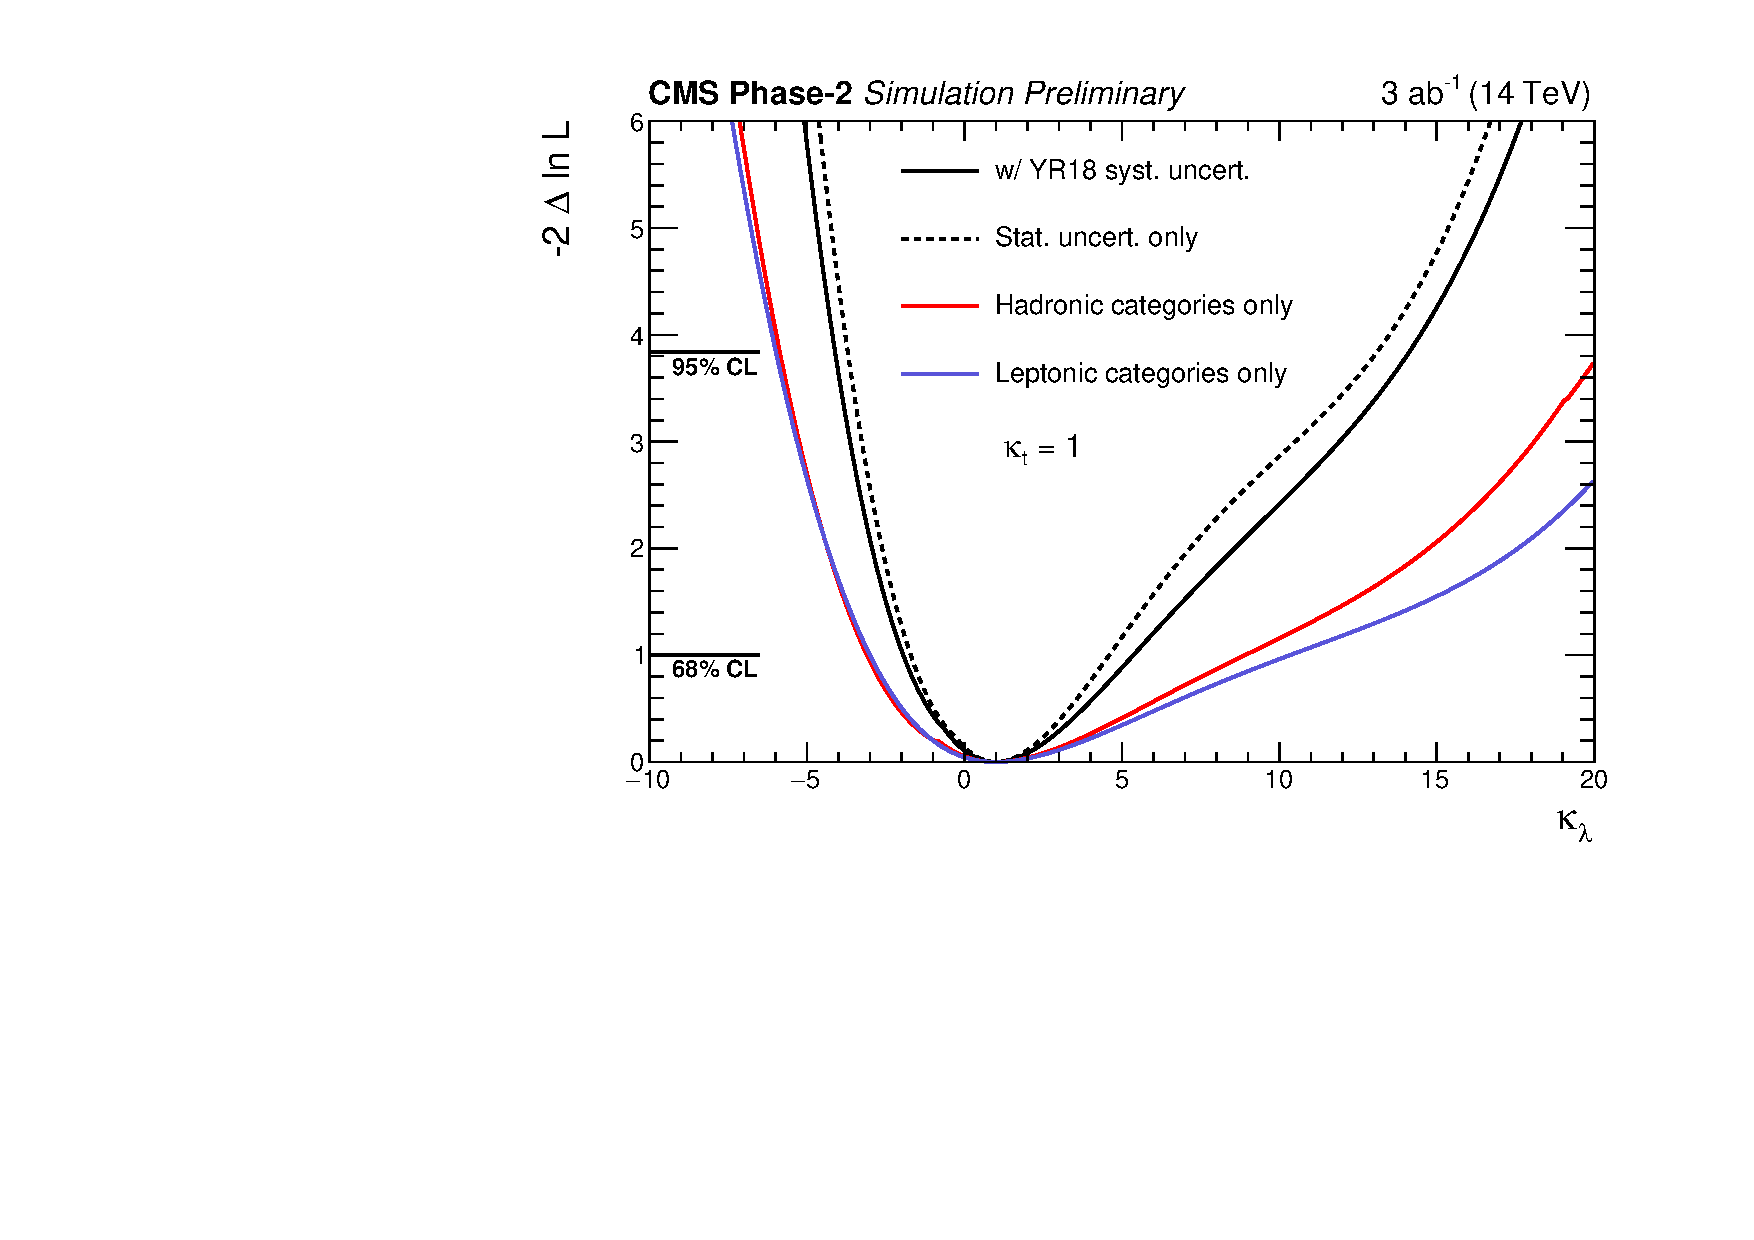
\includegraphics[width=0.6\textwidth]{\main/section3/plots/klambda_scan.pdf}
        %\vspace{2mm}
        \caption{Profile log-likelihood scan as a function of $\kappa_\lambda$. The individual contributions of the statistical and systematic uncertainties are separated by performing a likelihood scan with all systematics removed. Additionally, the contributions from the hadronic and leptonic channels have been separated, shown in red and purple, respectively.}
        \label{fig:ttHdiff_CMS_klambda_scan}
\end{figure}


The profiled log-likelihood in the region around 
$5<\kappa_\lambda<15$ results from the behaviour of the parametrisations which modify the predicted cross sections. For the $\ttH$ production mode, the derivative of the predicted cross section with respect to $\kappa_\lambda$ changes sign in this region, such that the predicted cross section is relatively stable for different values of $\kappa_\lambda$. This degeneracy is however somewhat resolved by the  other production modes for which the change in sign occurs at different values of $\kappa_\lambda$. With $3\,\text{ab}^{-1}$ of data collected by CMS at the HL-LHC, this result shows that a constraint of $-4.1 < \kappa_\lambda < 14.1$ at the 95\% confidence level (CL) is achievable from the differential cross-section measurement of a single Higgs boson decay channel produced in association with tops, using data from only one of the two general purpose detectors at the HL-LHC.  


The $\ttH$~+~$\tH$ differential cross section measurements are also sensitive to other potential BSM effects, such as those which give rise to anomalous top--Higgs couplings. A two-dimensional profile log-likelihood scan is shown in  Fig.~\ref{fig:ttHdiff_CMS_klambda_2Dscan} as a function of $\kappa_\lambda$ and $\mu_{H}$. The parameter $\mu_{H}$ is a multiplicative scaling factor which is common to all Higgs boson production modes and all $\pTH$ bins. Even with this additional parameter, constraints on $\kappa_\lambda$ are still achievable, owing to the information retained in the shape of the $\pTH$ distribution. The constraint on $\kappa_\lambda$ is $-7.1 < \kappa_\lambda < 14.1$ at the 95\% CL, when the log-likelihood is also profiled with respect to $\mu_{H}$. 

\begin{figure}[htb!]
        \centering
        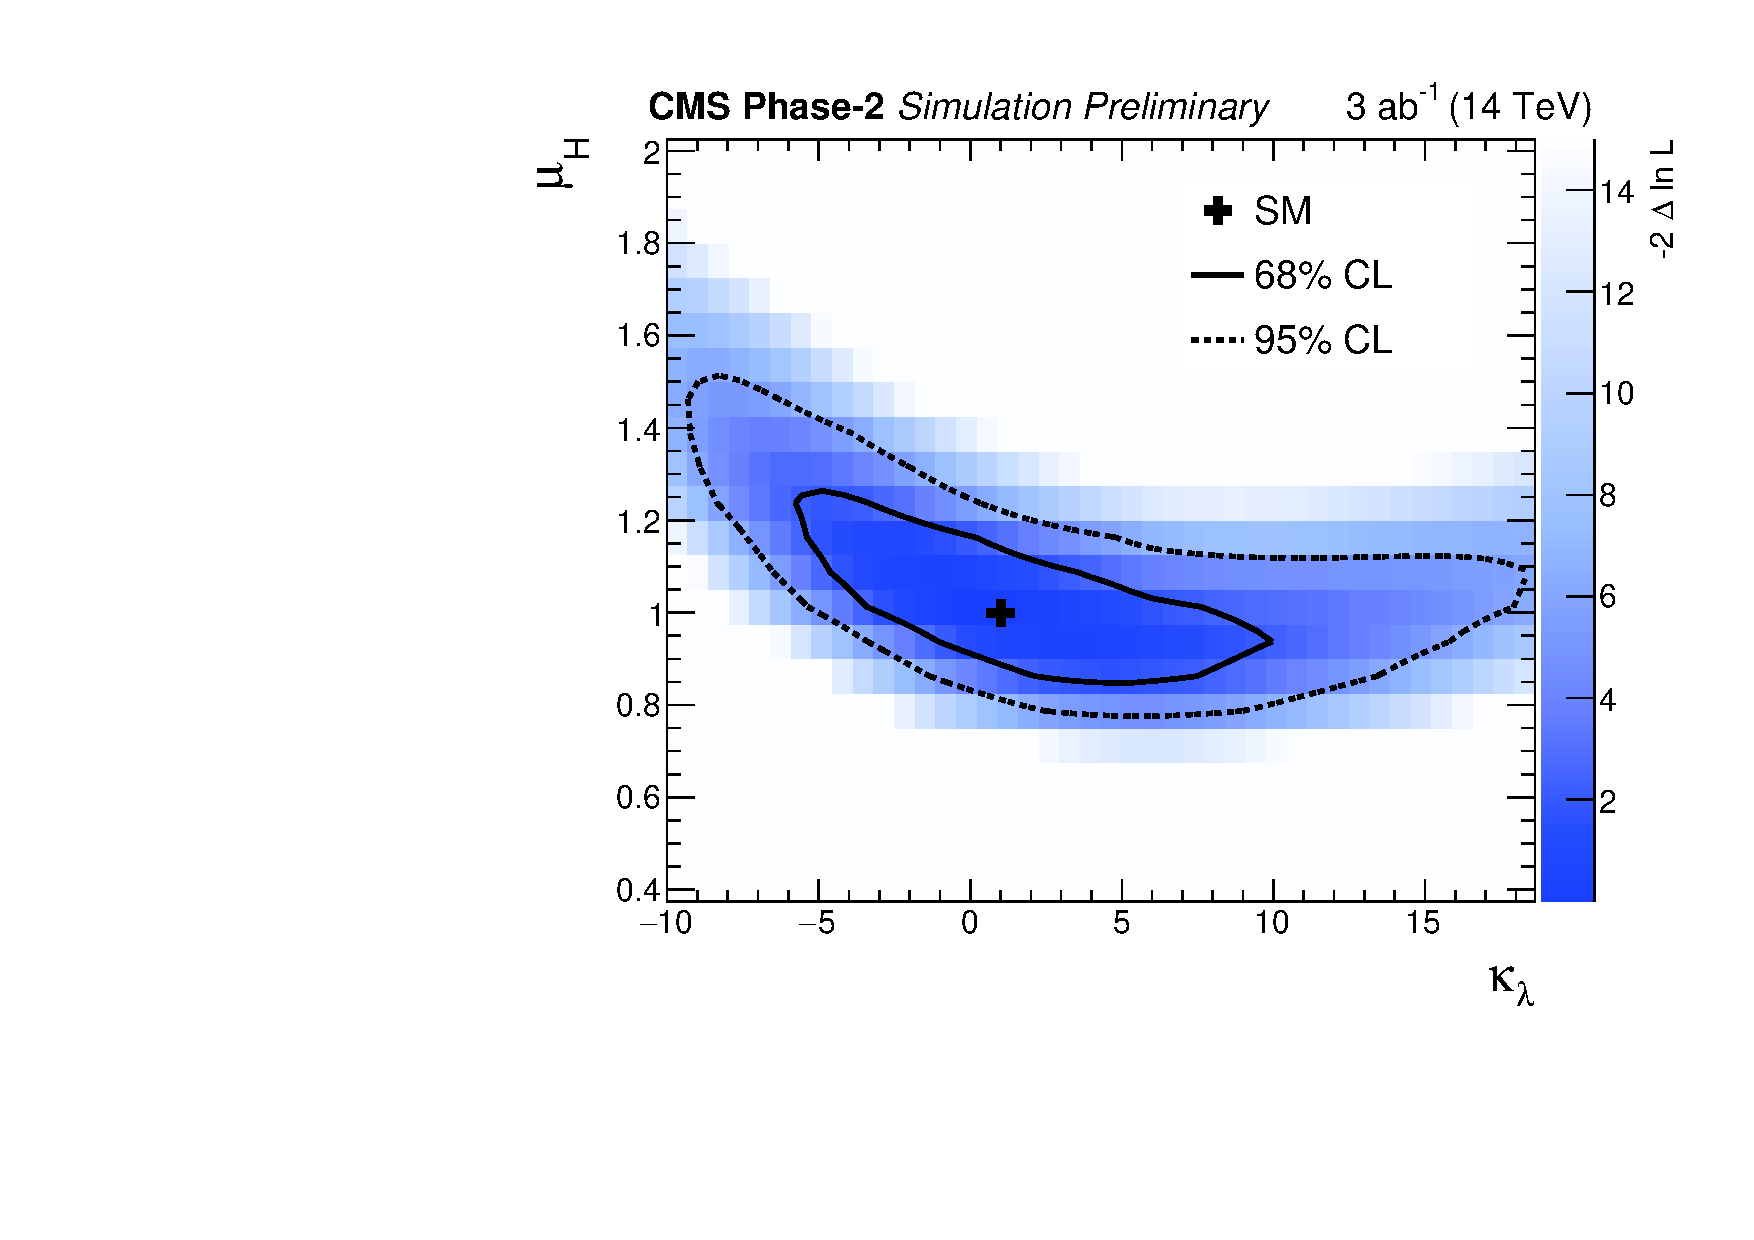
\includegraphics[width=0.6\textwidth]{\main/section3/plots/2D_kappa_mu_scan.pdf}
        %\vspace{2mm}
        \caption{Results of the two-dimensional likelihood scan in $\kappa_\lambda$-vs-$\mu_{H}$, where $\mu_{H}$ allows all Higgs boson production modes to scale relative to the SM prediction. The 68\% and 95\% confidence level contours are shown by the solid and dashed lines respectively. The SM expectation is shown by the black cross.}
        \label{fig:ttHdiff_CMS_klambda_2Dscan}
\end{figure}


